\chapter{Introduzione}
\label{section:intro}

\section{Il problema}
\label{section:problem_section}

In ambito universitario è problematica molto comune quella di dover assegnare aule a 
gruppi di studenti in modo tale da rispettare le richieste in numero di posti
di ciascuno di essi; questo senza nemmeno concretamente conoscere il numero di allievi che frequenteranno 
realmente il corso in questione, dovendo l'istituto assegnarle in anticipo rispetto all'inizio
delle lezioni.

Si pone quindi l'ulteriore problema di facilitare la raccolta di dati che permetta di effettuare 
delle stime più accurate, cioè di registrare in modo automatico la partecipazione degli universitari
a ciascuna lezione per inferire queste stime.

\medskip

Quest'applicazione si pone l'obiettivo di risolvere esattamente questa problematica (il funzionamento è 
illustrato in \ref{fig:app_flow});
a partire da foto (che si intende essere di aule) viene individuato il numero di volti e quindi di studenti in essa 
presenti: questo, associato ad ulteriori informazioni riguardanti la lezione in questione, viene fornito 
ad uno stimatore che, in base ai dati raccolti, cerca di costruire un modello matematico 
capace di prevedere il flusso di allievi nelle nuove situazioni richieste. Le stime verranno allora impiegate 
per distribuire ciascun gruppo nelle diverse aule con data capacità in modo ottimale, cercando cioè di 
massimizzare il valore di una certa funzione matematica che rappresenta il problema di allocazione. 

\begin{figure}
    \begin{small}
        \begin{center}
            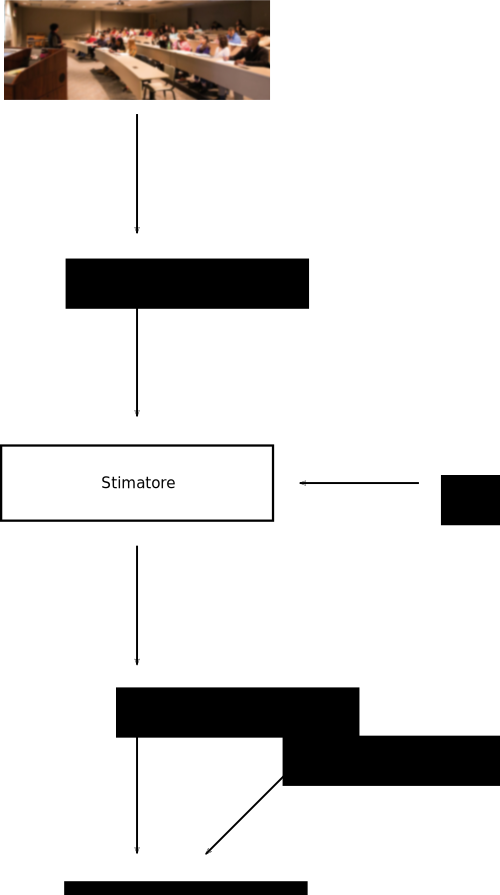
\includegraphics[width=0.70\textwidth]{app_flow.pdf}
        \end{center}
        \caption{Il flusso di funzionamento dell'applicazione}
        \label{fig:app_flow}
    \end{small}
\end{figure}

\section{Struttura del documento}
\label{section:doc_structure}

Il documento è strutturato in 

\begin{itemize}
    \item \textbf{\nameref{section:state_of_the_art}}, in cui vengono inizialmente accennati i concetti teorici utilizzati per la risoluzione 
        del problema su argomenti quali
        \begin{enumerate}
            \item \textbf{\nameref{section:face_detection}}
            \item \textbf{\nameref{section:regression_ml}} 
            \item \textbf{\nameref{section:lin_programming}}; 
        \end{enumerate}

        vengono quindi analizzati articoli e pubblicazioni che hanno affrontato le stesse problematiche 
        (\textbf{\nameref{section:past_works}}).
        
    \item \textbf{\nameref{section:methods}}, nel quale sono approfondite le metodologie usate per la realizzazione 
        dell'applicazione (capitoli \ref{section:methods_face_detection}, \ref{section:methods_ml} e \ref{section:methods_allocation})
    \item \textbf{\nameref{section:results}}, che illustra gli esiti e l'efficienza ed un'analisi della realizzazione scelta (capitolo 
        \ref{section:results})
    \item \textbf{\nameref{section:conclusion}}, contenente le osservazioni finali dedotte insieme all'illustrazione di possibili 
        miglioramenti.
\end{itemize}

\section{Codice sorgente}

Il codice completo di questa applicazione è accessibile su GitHub al seguente 
indirizzo 

\begin{center}
    \url{https://github.com/morpheusthewhite/celephais}; 
\end{center}

\noindent
analogamente è stato pubblicato il codice \LaTeX di questa tesi al link 

\begin{center}
    \url{https://github.com/morpheusthewhite/bachelor-thesis}.     
\end{center}
